\documentclass{book}

\usepackage{Typocaps,lettrine}
\usepackage{graphicx,float}
\usepackage{subfig}
\usepackage{amsmath, amsthm, amsfonts, amssymb, mathtools}
\usepackage[export]{adjustbox}
\usepackage{enumitem}
\usepackage{chapterbib}
\usepackage[ruled]{algorithm2e}
\usepackage{caption}
\usepackage{float}
\newcommand{\N}{\mathbb{N}}
\renewcommand{\qedsymbol}{$\blacksquare$}
\renewcommand\LettrineFontHook{\Typocapsfamily}

\DeclarePairedDelimiter\abs{\lvert}{\rvert}%
\DeclarePairedDelimiter\norm{\lVert}{\rVert}%

\newtheorem{theorem}{Theorem}[chapter]
\newtheorem{corollary}{Corollary}[theorem]
\newtheorem{lemma}[theorem]{Lemma}

\theoremstyle{definition}
\newtheorem{definition}{Definition}[section]

\title{The little book of graph notes}
\author{Graph theory students}

\begin{document}
\maketitle
\tableofcontents

\section*{Preface}
This compilation of notes exists as a project for students in the CMSC 420 Graph Theory course at Longwood University. These notes have been created by all the students of the class, and an attempt has been made to both categorize the notes in a logical, sequential manner, and to ensure that the information is clear yet concise.

% \chapter{A starting point}
\lettrine[lines=4]{G}{raphs} do things and stuff.  They have recieved a great
deal of attention lately because they can model real world \textit{relationships}.  But what is
a graph?  

\includegraphics[width=0.4\textwidth]{tree.pdf}

\begin{figure}%
    \centering
    \subfloat[k5]{{\includegraphics[width=0.4\textwidth]{k5.pdf} }}%
    \qquad
    \subfloat[k5 again]{{\includegraphics[width=0.4\textwidth]{k5.pdf} }}%

    \subfloat[k5 again]{{\includegraphics[width=0.4\textwidth]{k5.pdf} }}%
    \caption{side by side graphs}%
    \label{fig:k5}%
\end{figure}


\chapter{On Graphs}
\section{What is a Graph?}
\lettrine[lines=4]{G}{raphs}, in their elementary form, are a pair of sets: $V$ (\textbf{Vertices}) and $E$ (\textbf{Edges}) such that $V \neq \emptyset$ ($V$ cannot be empty), and $\forall e \in E, e = \{v_i, v_j\}, v_i, v_j \in V$ (every edge in $E$ is a pairwise subset of vertices $v_i$ and $v_j$ in $V$). Here is an example of a very simple graph:

\begin{center}
    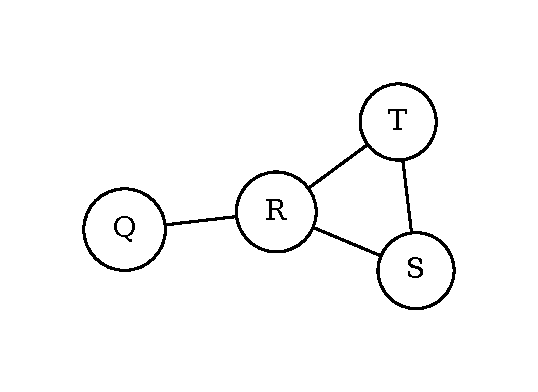
\includegraphics[width=0.5\textwidth]{Chapter1/graph.pdf}
\end{center}

In this graph, our vertex set is $V = \{Q, R, S, T\}$, and our edge set is $E = \big\{\{Q, R\}. \{R, S\}, \{R, T\}, \{S,T\}\big\}$.

Other names for Vertices are \textbf{nodes} or \textbf{points}. Other names for edges are \textbf{links} or \textbf{lines}. When we want to refer to the vertex set of a specific graph $G$, we will denote it as $V(G)$. Similarly, we will denote the edge set as $E(G)$.
\section{Why do we care about Graphs?}
Graphs can be used to model many real world problems, or theoretical ideas. For example, graphs can be used to represent relationships between different objects or groups. They are useful for visualizing data, such as social media connections, or network topology. Additionally, a more practical use is for mapping routes from one location to another, much like the GPS on your phone.

As for more theoretical uses, graphs can represent other structural relationships. Tree structures are a type of graph, as are flow diagrams or DFAs/NFAs from Computation Theory. Perhaps one of their more important uses is in determining where problems fit in P vs. NP.

\section{On Different Types of Graphs}
\subsection{Multigraphs}
A \textbf{multigraph} is a pair of sets $(V, E)$ such that $V \neq \emptyset$, and $E$ is a finite family of unordered pairs of $V$. That is to say, edges are not necessarily unique subsets, and do not have order. Thus, multigraphs allow for loops from one vertex to itself. Here is an example of a multigraph:

\begin{center}
    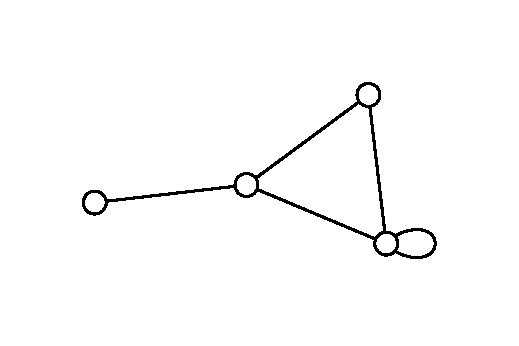
\includegraphics[width=0.5\textwidth]{Chapter1/multigraph.pdf}
\end{center}

Because multigraphs are unordered, then an edge $(a, b)$ would be the same as $(b, a)$. But what if we only want an edge in one direction but not the other?
\subsection{Digraphs}
A \textbf{digraph} is a pair of sets $(V, E)$ such that $V \neq \emptyset$, and $E$ is a set of ordered pairs of elements in $V$. Informally, we say that a digraph is a directed graph, where we annotate each edge with an arrow to mark the direction it flows. Here is an example of a digraph:

\begin{center}
    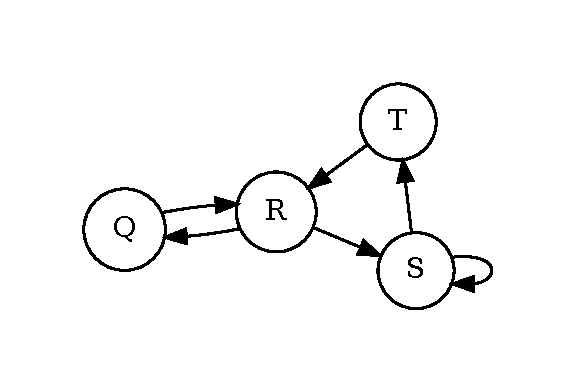
\includegraphics[width=0.5\textwidth]{Chapter1/digraph.pdf}
\end{center}

\section{On Vertices and Edges}
There is a lot to be said of the mathematics of graphs, but before we can establish such mathematics, we must first establish some essential definitions. Let $G$ be a graph with vertex set $V$ and edge set $E$. Let $u, v, w \in V$ be vertices of $G$.
\begin{description}
    \item[Join:] If $\{u, v\} \in E$, then $u$ is said to \textbf{join} $v$.
    \item[Adjacent:] $u$ and $v$ are said to be \textbf{adjacent} if $\{u, v\} \in E$. Similarly, if $\{u, v\}, \{u, w\} \in E$, then $\{u, v\}$ and $\{u, w\}$ are said to be \textbf{adjacent}.
    \item[Incident:] If $\{u, v\} \in E$, then $u$ and $v$ are said to be \textbf{incident} to $\{u, v\}$. Similarly, if $\{u, v\}, \{u, w\} \in E$, then $\{u, v\}$ and $\{u, w\}$ are said to be \textbf{incident} to $u$.
    \item[Degree:] The \textbf{degree} of a vertex, denoted deg($v$) or $\rho(v)$, is the number of edges incident to $v$.
    \item[Isolated:] If deg($v$) = 0, then we say $v$ is an \textbf{isolated} vertex.
    \item[Pendant:] If deg($v$) = 1, then we say $v$ is a \textbf{pendant} vertex.
\end{description}
These are a lot of formal definitions, but they will be useful when classifying different graphs and discussing their structures and properties. Informally, we say two edges are adjacent if they share a vertex, and two vertices are adjacent if they share an edge. Similarly, we say that two edges are incident to a vertex if they share that vertex, and two vertices are incident to an edge if they share that edge. 

\section{On Isomorphisms}
The term \emph{isomorphic} has its roots in Greek, \emph{iso-} meaning same, and \emph{morphic} referring to form or shape. We say that two graphs are \textbf{isomorphic} if they have this ``same shape'' property, but what does that mean?

Mathematically, we say that the graph $G_1$ is \textbf{isomorphic} to the graph $G_2$, denoted $G_1 \sim G_2$, if there is a one-to-one correspondence between the vertices $V_1$ of $G_1$ and the vertices $V_2$ of $G_2$ that preserves adjacencies. This is a mapping $f$ from $G_1$ to $G_2$ defined as follows:
\begin{center}
    $f : G_1 \mapsto G_2$ such that $\forall \{v_i, v_j\} \in E(G_1), \{f(v_i), f(v_j)\} \in E(G_2)$
\end{center}
This may look like a lot of intimidating gibberish, but it represents the idea of preserving the edges between two vertices in $G_1$ after mapping them to $G_2$. For example, the following graphs are isomorphic:
\begin{center}
    \includegraphics[width=0.4\textwidth]{Chapter1/isomorphicA.pdf} % Compile isomorphic.dot with neato
    \includegraphics[width=0.4\textwidth]{Chapter1/isomorphicB.pdf} % Compile isomorphic.dot with circo
\end{center}
Isomorphisms are a mapping, and thus have certain propoerties that allow us to classify them with other mappings. Let $G_1, G_2,$ and $G_3$ be graphs. Isomorphisms are what we call an equivalence relation, as the following three propoerties hold:
\begin{description}
    \item[Reflexive:] $G_1 \sim G_1$
    \item[Symmetric:] If $G_1 \sim G_2$, then $G_2 \sim G_1$
    \item[Transitive:] If $G_1 \sim G_2$ and $G_2 \sim G_3$, then $G_1 \sim G_3$
\end{description}

\subsection{The Handshaking Lemma}
We are now armed with enough information to decipher some information hidden in the graphs we deal with. The first of these is called the Handshaking Lemma. Let's tackle this proof:

\begin{lemma}[The Handshaking Lemma]
    Let $G$ be a graph. Then the number of vertices with odd degree is even.
\end{lemma}
\begin{proof}
    Let $V = \{v_1, v_2, \ldots, v_n\}$ be the vertices of $G$. The the sum of the degrees,
    \begin{equation*}
        \sum_{i=1}^n \text{deg}(v_i) = 2m, m \in \mathbb{Z},
    \end{equation*}
    is even, since each edge is counted twice (convince yourself that this must be true, if you don't understand). Now, if we were to remove all vertices of even degree, then we would be removing an even number of edges from this sum. This leaves us with
    \begin{equation*}
        \sum_{odd~degrees}^n \text{deg}(v_i) = 2k, k \in \mathbb{Z},
    \end{equation*}
    which is even. Now, the only way for the sum of odd numbers to be even is for there to be an even number of those odds. Thus, we must have an even number of odd degree vertices in $G$.
\end{proof}
\section{On Special Kinds of Graphs}
We've talked a lot about the different aspects of graphs, but now let's use this information to actually classify different kinds of graphs, starting with the \textbf{null graph}. the null graph is a graph with $n$ vertices but no edges, and is denoted as $N_n$.

A \textbf{regular graph} is a graph $G$ with $n$ vertices whose vertices all have the same degree, and we say such a graph is regular of degree $r < n$.

A \textbf{complete graph} is a graph $G$ with $n$ vertices that is regular of degree $n-1$. We denote such a graph by $K_n$. The total number of edges in the complete graph $K_n$ is given by summing the number of edges: 
\begin{equation*}
    \sum_{i=1}^{n-1} i = \frac{(n-1)(n-2)}{2}
\end{equation*}

A \textbf{bipartite graph} is a graph with vertex set $V = V_1 \cup V_2$ where $V_1 \cap V_2 = \emptyset$ and $\forall v_i, v_j \in V_1$ and $v_m, v_n \in V_2$, $(v_i, v_j), (v_m, v_n) \not\in E$. This is another way to say that the vertices of a bipartite graph $G$ can be divided into two sets there all edges in $G$ only go between both sets - neither set of vertices has two vertices which make an edge. A complete bipartite graph is denoted $K_{m, n}$, with two sets containing $m$ and $n$ vertices, with all vertices in one set connecting to all the vertices of the other. Here is an example of a bipartite graph, $K_{3, 3}$:
\begin{center}
    \includegraphics[width=0.3\textwidth]{Chapter1/isomorphicB.pdf}
\end{center}

A \textbf{subgraph} of $G = (V, E)$ has the vertex set $H$ and the edge set $F$, where $H \subseteq V$ and $F \subseteq E$, but only the edges of $E$ which correspond to the vertices in $H$ can be in $F$.

\section{On the Storage of Graphs}
We've talked a lot about graphs and their theories and applications, but how exactly do we represent graphs in a computer? The idea that a graph defines a set of relations in important, so the natural way to consider this is some sort of data structure with nodes which point to their adjacent neighbors. This certainly is an intuitive way to consider this, but examining them mathematically will make our lives easier in the future.

Consider the following graph:
\begin{center}
    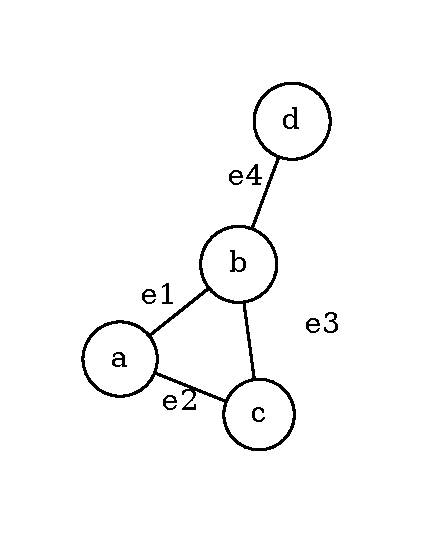
\includegraphics[width=0.5\textwidth]{Chapter1/mat.pdf}
\end{center}
We can store this in what's called an \textbf{Adjacency Matrix}, a matrix where each row and column represents a particular vertex in the graph, and entries in the matrix signify that two vertices share an edge. The adjacency matrix for the given graph is:
\begin{center}
    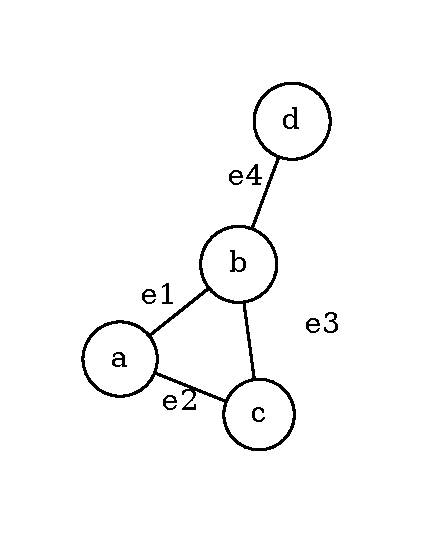
\includegraphics[width=0.4\textwidth]{Chapter1/mat.pdf} $\bordermatrix{~ & a & b & c & d \cr
                                                                           a & 0 & 1 & 1 & 0 \cr
                                                                           b & 1 & 0 & 1 & 1 \cr
                                                                           c & 1 & 1 & 0 & 0 \cr
                                                                           d & 0 & 1 & 0 & 0 }$
\end{center}
We usually denote an adjacency matrix $[A_{i, j}]$, where a 1 in entry $a_{i, j}$ identifies that vertices $i$ and $j$ share an edge, and a 0 means that they don't. While adjacency matrices for a graph with $n$ vertices occupies $n^2$ space, they do provide constant lookup time to see if two vertices share an edge.

We also have an \textbf{Incidence Matrix}, which tells us if an edge and a vertex are incident. The incidence matrix for the graph above is:
\begin{center}
    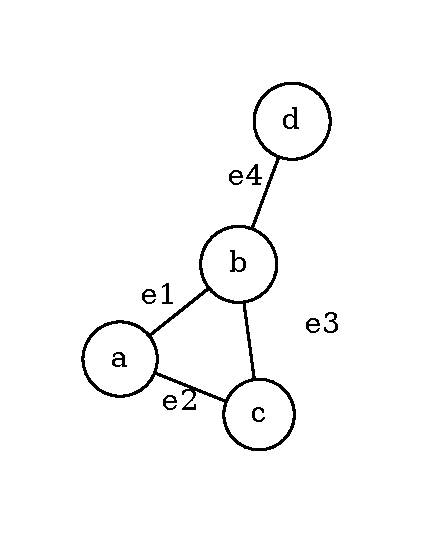
\includegraphics[width=0.4\textwidth]{Chapter1/mat.pdf} $\bordermatrix{~ & e_1 & e_2 & e_3 & e_4 \cr
                                                                           a & 1 & 1 & 0 & 0 \cr
                                                                           b & 1 & 0 & 1 & 1 \cr
                                                                           c & 0 & 1 & 1 & 0 \cr
                                                                           d & 0 & 0 & 0 & 1 }$
\end{center}
It might be preferable to use the adjacency matrix for the symmetry along the main diagonal of the matrix. 
% \chapter{Forest for the trees}
\lettrine[lines=4]{T}{rees} are just graphs. There are lots more to say about trees but that is
your job not mine. I already said some stuff once. 


\chapter{Forest for the Trees}
\lettrine[lines=4]{T}{rees} are another special kind of graph which we did not discuss in the previous chapter. Trees are somewhat unique compared to the other types of specialty graphs described before as they allow us certain algorithms to perform to solve different problems. Before we go in depth into trees, we must first define an operation and some other terms.

\section{Definitions}
Let $G_1$ and $G_2$ be graphs. Then $G_1 \cup G_2$ is the \textbf{union} of $G_1$ and $G_2$ with the vertex set $V = V(G_1) \cup V(G_2)$ and edge set $E = E(G_1) \cup E(G_2)$. Now, let's establish some more definitions:
\begin{description}
    \item[Disconnected:] A graph is \textbf{disconnected} if it is the union of two graphs. Here is an example of a disconnected graph:
    \begin{center}
        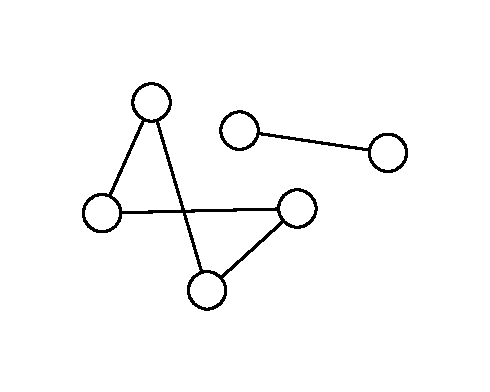
\includegraphics[width=0.3\textwidth]{Chapter2/disconnect.pdf}
    \end{center}
    \item[Connected:] A graph is \textbf{connected} if it is not disconnected (wow). Here is an example of a connected graph:
    \begin{center}
        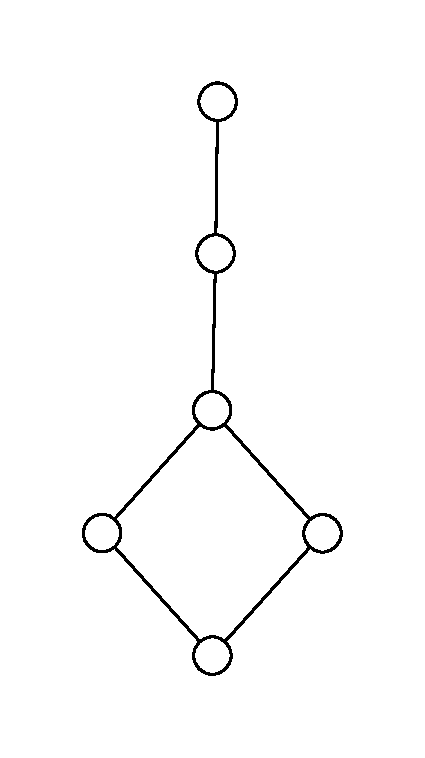
\includegraphics[width=0.3\textwidth]{Chapter2/connect.pdf}
    \end{center}
    \item[Component:] A \textbf{component} graph is one graph which makes up part of a union. In $G = G_1 \cup G_2$, $G_1$ and $G_2$ are components.
\end{description}

We can also define the \textbf{subtraction} of a set of edges $F$ from a graph $G$. We say that $G - F$ is the graph resulting in the removal of the edges in $F$ from $G$. Suppose we have the following graph $G$:
\begin{center}
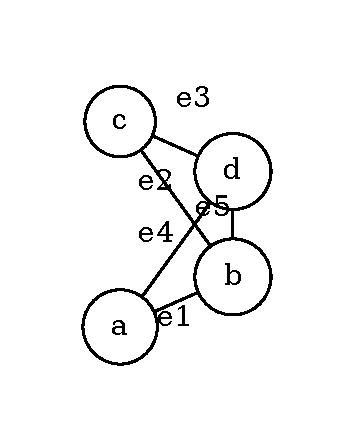
\includegraphics[width=0.3\textwidth]{Chapter2/sub0.pdf}
\end{center}
Then the following are different subtractions from $G$.
\begin{figure}[h]
    \subfloat[$G - \{e1\}$]{
        \begin{minipage}[c][1\width]{0.3\textwidth}
            \centering
            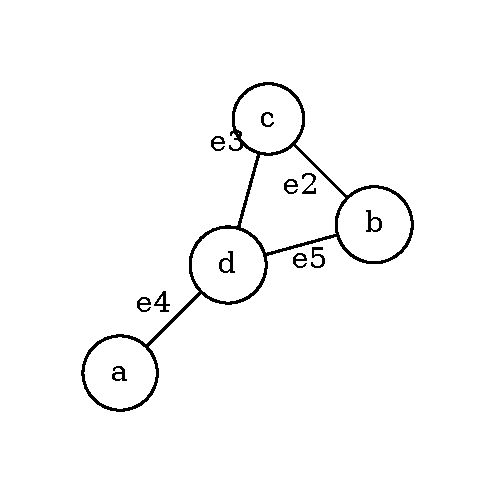
\includegraphics[width=1.\textwidth]{Chapter2/sub1.pdf}
        \end{minipage}
    }
    \subfloat[$G - \{e2\}$]{
        \begin{minipage}[c][1\width]{0.3\textwidth}
            \centering
            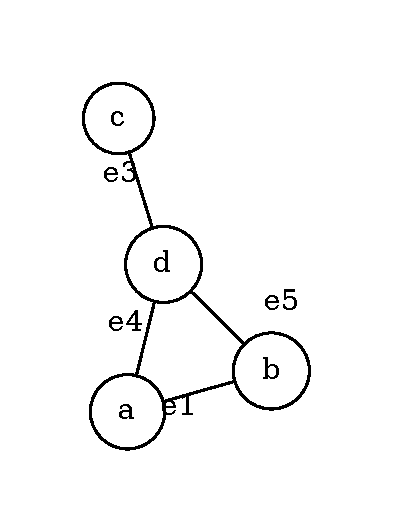
\includegraphics[width=\textwidth]{Chapter2/sub2.pdf}
        \end{minipage}
    }
    \subfloat[$G - \{e1, e2\}$]{
        \begin{minipage}[c][1\width]{0.3\textwidth}
            \centering
            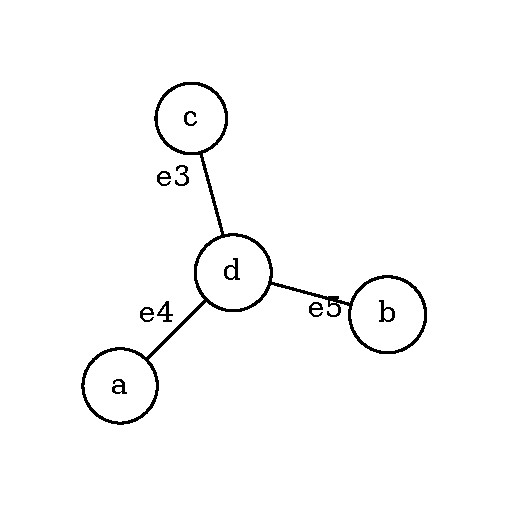
\includegraphics[width=\textwidth]{Chapter2/sub12.pdf}
        \end{minipage}
    }
\end{figure} 

Let's define a new type of graph. A connected graph that is regular of degree 2 is called a \textbf{cycle}, which we denote $C_n$. Here is an example of a cycle, $C_5$:
\begin{center}
    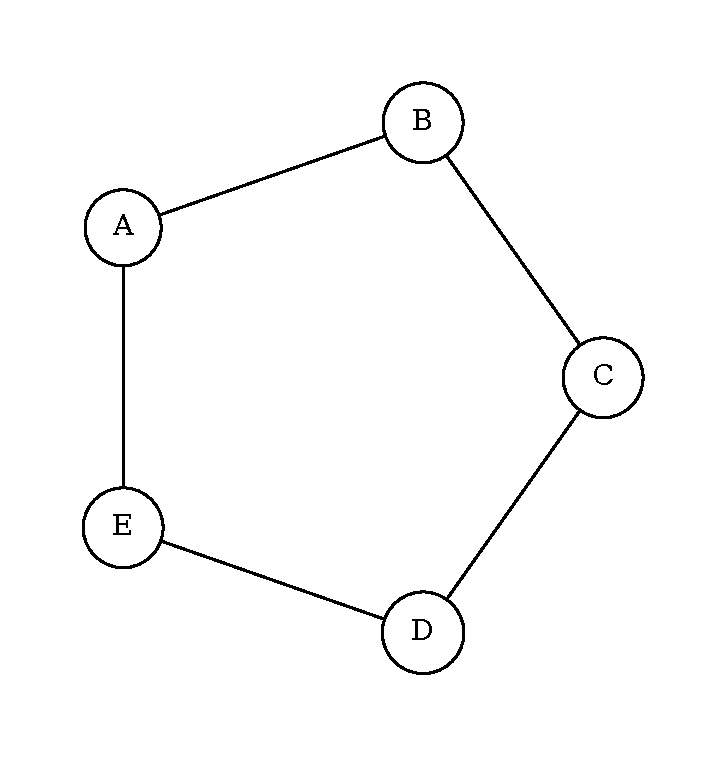
\includegraphics[width=0.3\textwidth]{Chapter2/c5.pdf}
\end{center}

A useful operation on graphs is to take the complement. The \textbf{complement} of a graph $G$ is the graph $\overline{G}$, with vertex set $V(\overline{G}) = V(G)$, with two vertices adjacent in $\overline{G}$ if and only if they are \emph{not} adjacent in $G$. Given $C_5$, we can fine its complement, $\overline{C_5}$:
\begin{center}
    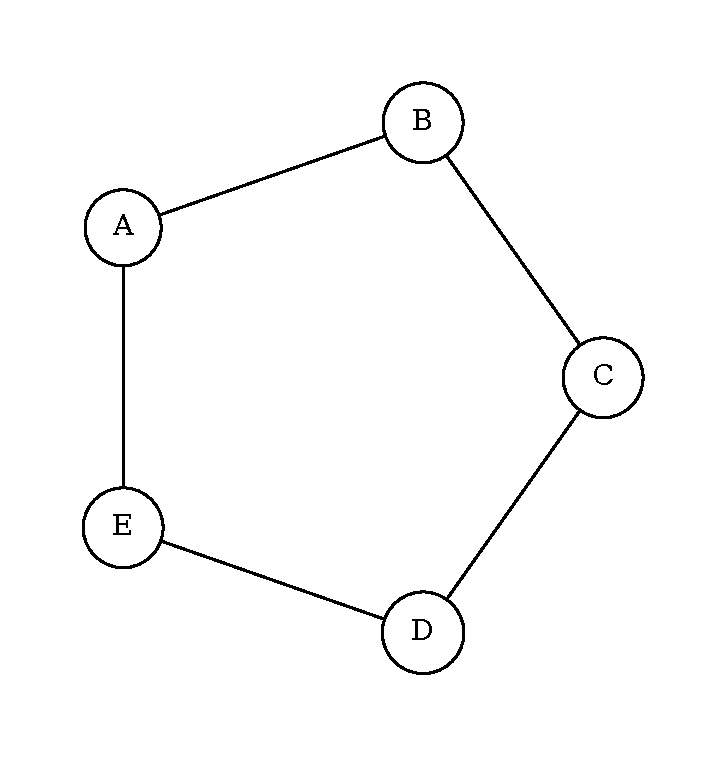
\includegraphics[width=0.3\textwidth]{Chapter2/c5.pdf}
    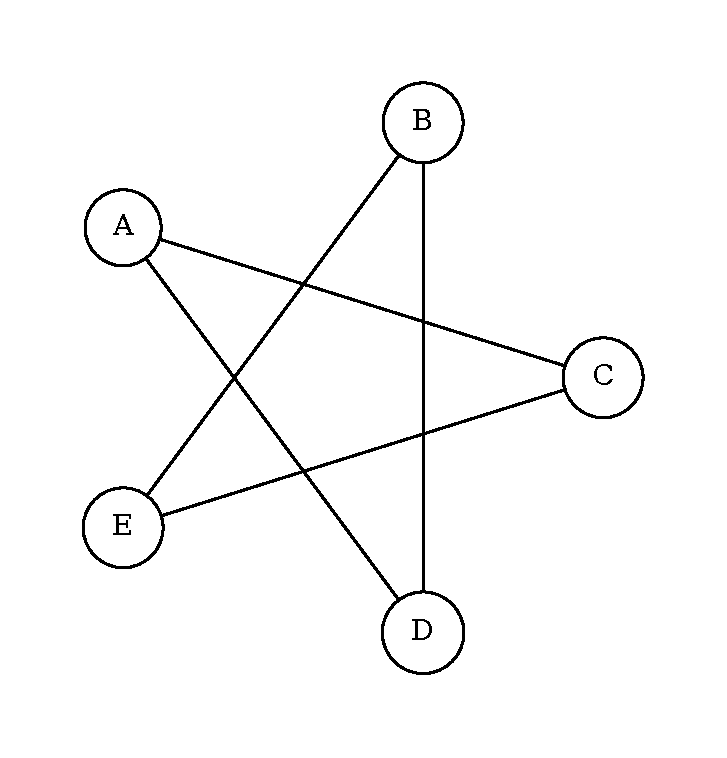
\includegraphics[width=0.3\textwidth]{Chapter2/c5comp.pdf}
\end{center}
In this particular example, notice that $C_5 \sim \overline{C_5}$, so $C_5$ is what we call \textbf{self-complementary} - it is isomorphic to its own complement.

\section{Trailblazing}
We've defined what graphs are as a construct, but how do we actually navigate from one point to another? There are different ways to navigate from vertex to vertex, and each form of navigation takes on different attributes. Consider the following graph $G_0$:
\begin{center}
    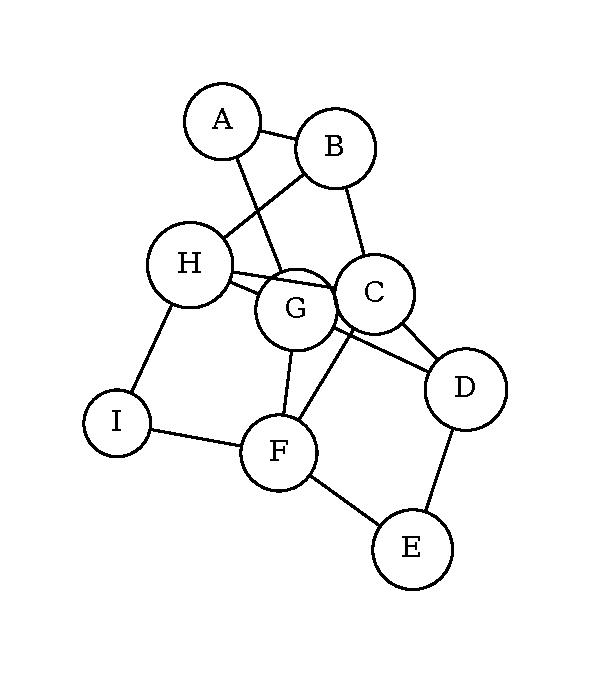
\includegraphics[width=0.5\textwidth]{Chapter2/nav.pdf}
\end{center}
Let's define some of the different ways we can navigate through $G_0$:
\begin{description}
    \item[Walk:] A \textbf{walk} in a graph $G$ is any finite sequence of edges, $v_0v_1, v_1v_2, v_2v_3, \ldots, v_{k-1}v_k$. The initial vertex is denoted $v_0$, and the final vertex is denoted $v_k$. The \textbf{length} of the walk is $k$. Here is an example of a walk in $G_0$:
    \begin{center}
        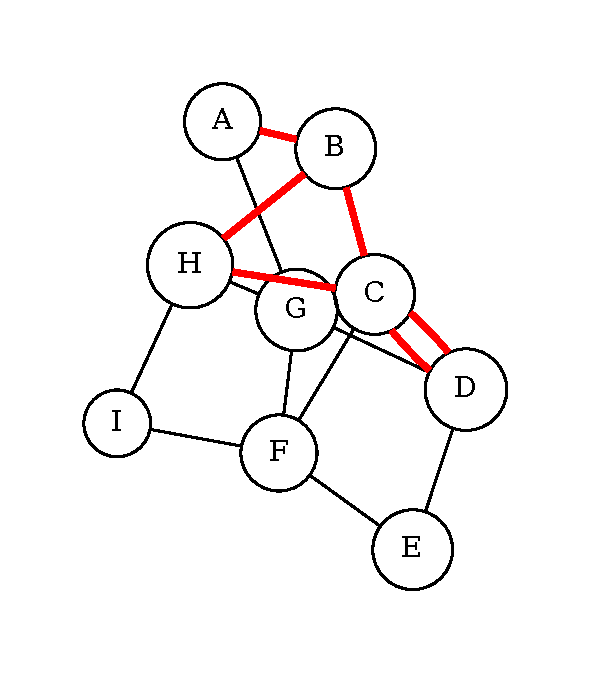
\includegraphics[width=0.5\textwidth]{Chapter2/walk.pdf}
    \end{center}
    Here, the walk shown begins at node $A$. The walk is $AB, BH, HC, CD, DC$, $CB$. The length of this walk is 6.
    \item[Trail:] A walk where all the \emph{edges} are distinct is a \textbf{trail}. The walk observed above is not a trail, since the edge $\{C, D\}$ is repeated. Thus, a variation of this as a trail might be:
    \begin{center}
        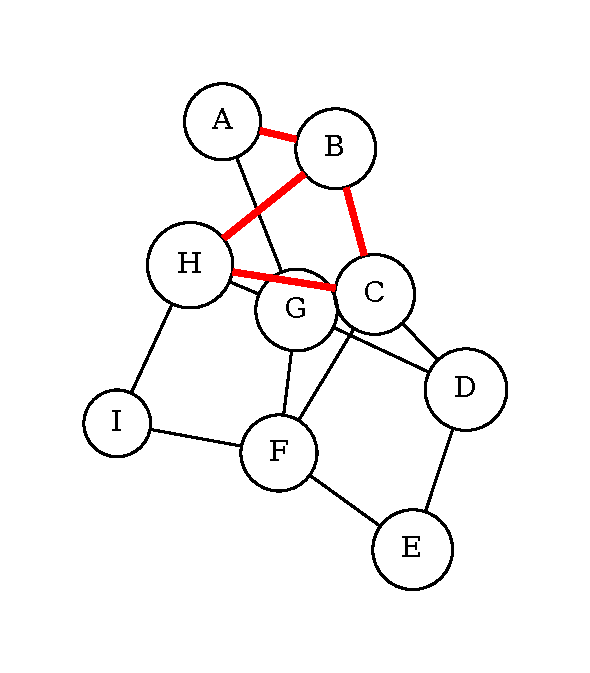
\includegraphics[width=0.5\textwidth]{Chapter2/trail.pdf}
    \end{center}
    The trail here is $AB, BH, HC, CB$.
    \item[Path:] A trail where all the \emph{vertices} are unique is called a \textbf{path}. The trail above would not be a path, as the vertex $B$ is visited twice. Here is an example of a path in $G_0$:
    \begin{center}
        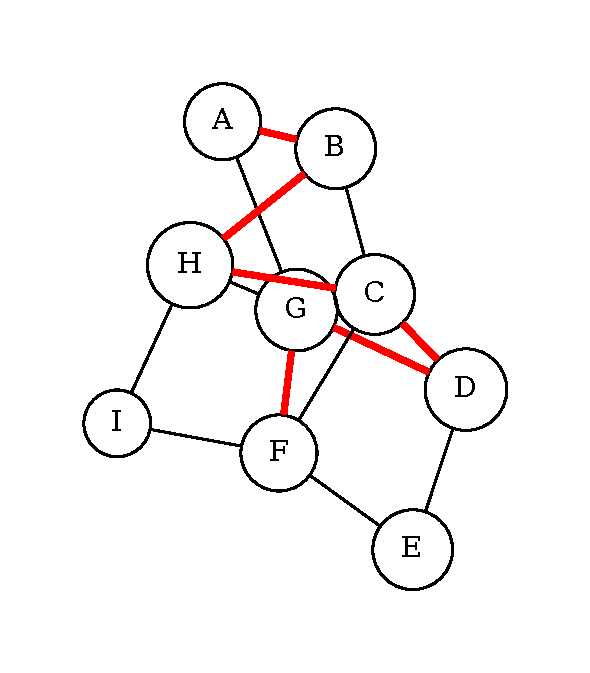
\includegraphics[width=0.5\textwidth]{Chapter2/path.pdf}
    \end{center}
    This path is $AB, BH, HC, CD, DG, GF$.
    \item[Cycle:] A \textbf{closed} path (where $v_0 = v_k$) has at least one edge, then it is a \textbf{cycle}. Here is an example of a cycle in $G_0$:
    \begin{center}
        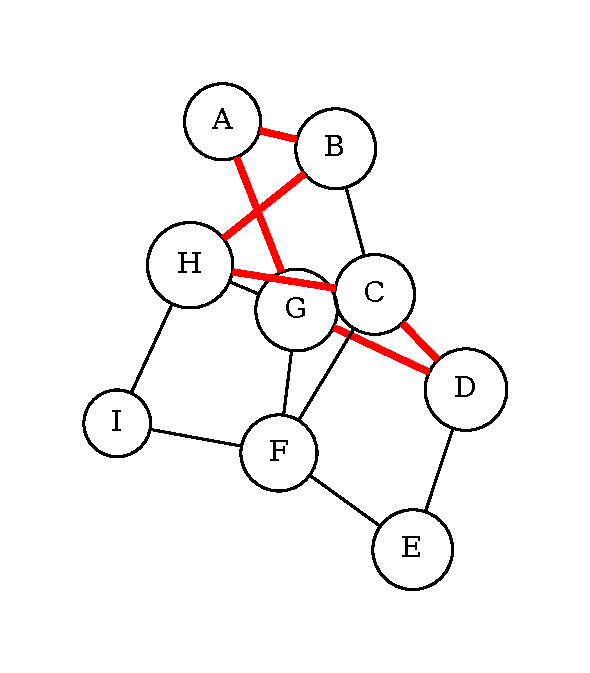
\includegraphics[width=0.5\textwidth]{Chapter2/cycle.pdf}
    \end{center}
    This cycle is $AB, BH, HC, CD, DG, GA$.     
\end{description}
\section{The Lorax}
We have the terminology we need to finally describe the subjects of this chapter: trees and forests. 
\begin{description}
    \item[Forest:] A \textbf{forest} is a graph with no cycles. It need not necessarily be connected, so long as there are no cycles. Here is an example of a forest:
    \begin{center}
        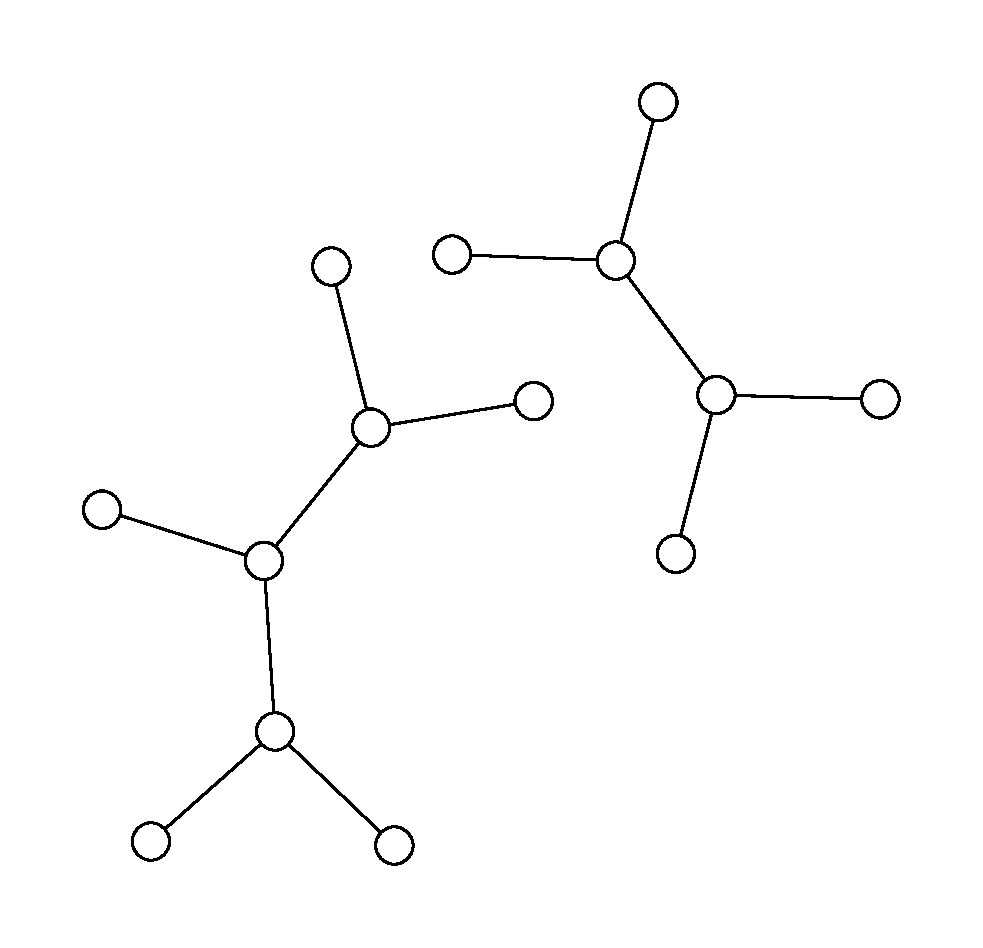
\includegraphics[width=0.5\textwidth]{Chapter2/forest.pdf}
    \end{center} 
    \item[Tree:] A \textbf{tree} is a connected forest. Here is an example of a tree:
    \begin{center}
        \includegraphics[width=0.5\textwidth]{Chapter2/tree.pdf}
    \end{center} 
\end{description}
Trees come in many different shapes and sizes, the count of which grows quickly as more nodes are introduces. For example, there is only one tree of one, two, and three nodes. Once we introduce a fourth node, we see that there are two distinct trees of four nodes. The more nodes we introduce, the more rapidly the count of distinct isomorphisms increases. 

\section{(Minimum) Spanning Trees}
While fundamentally trees and forests are just different kinds of graphs, they are useful tools when used in conjunction with graphs. One example of this is the \textbf{spanning tree} of a graph. The spanning tree of a graph $G$ is a tree which includes all vertices of the graph $G$. Another way to imagine this is a non-cyclic representation of $G$. On top of spanning trees, we have \textbf{minimum spanning trees} (MSTs). The MST of a graph $G$ is a spanning tree whose whose total weight is minimal compared to all spanning trees. First, let's define what a weight is.

A \textbf{weight} is a numerical value assigned to an edge. This number is representative of the total cost of traversing from one vertex to another along that particular edge - some edges may be cheaper, others may be longer. We assume that these weights are strictly non-negative (so for a weight $n, n \in \mathbb{Z}^*$). The total weight of a graph is the sum of the weights of all edges.

Again, the MST for a graph $G$ is a spanning tree with minimal weight. How do we find the minimum spanning tree for a graph? There are three popular algorithms which solve this problem: Prim's Algorithm, Kruskal's Algorithm, and Bor\r{u}vka's Algorithm.
\subsection{Prim's Algorithm}
Prim's Algorithm was originally developed by Czech mathematician Vojt\v{e}ch Jarn\'{i}k in 1930, but was later published by Robert Prim and Edsger Dijkstra in 1959\cite{PrimsAlgo}. Prim's algorithm focuses on the vertices of a graph, and considers edges incident to the vertices in the MST as it grows. Below is a quick pseudocode representation of this algorithm\cite{IntroToAlgo}.

\begin{algorithm}
    \DontPrintSemicolon
    \caption{Prim's Algorithm}

    \KwData{Weighted graph $G$, root vertex $v_0$}
    \KwResult{Minimum spanning tree $T$}
    \SetKwFunction{setw}{Weight}
    \SetKwFunction{setp}{Parent}
    \SetKwFunction{exmin}{GetMinVertex}
    \SetKwFunction{edge}{EdgeWeight}
    \SetKwFunction{adj}{AdjacentTo}

    \For{$v \in V(G)$}{
        \setw{v} $\gets \infty$\;
        \setp{v} $\gets$ null\;
    }
    \setw{$v_0$} $\gets 0$\;
    $Q \gets V(G)$\;
    \While{$Q \neq \emptyset$}{
        $u \gets$ \exmin{$Q$}\;
        \ForEach{$v \in$ \adj$(u)$}{
            \If{$v \in Q$ and \edge{$u, v$} $<$ \setw{$v$}}{
                \setp{$v$} $\gets u$\;
                \setw{$v$} $\gets$ \edge{$u, v$}
            }
        }
    }
\end{algorithm}

Given a root node $v_0$ to begin the construction of the MST, the objective for the algorithm is to construct a tree based on weights from nodes already examined. The preliminaries of this algorithm look very much like Dijkstra's algorithm (discussed later), where we initialize the weights of all vertices to infinity, and the root node to zero. Additionally, we want to keep track of the edge through which we reach the vertex, so we initialize the parent to null. 

We use $Q$ as a minimum heap structure to grab the smallest weighted vertex, calling it $u$. The idea is to examine all adjacent vertices to $u$, and update their current weight if following the edge from $u$ to said vertex is better than what was found previously. If so, we set the parent of that vertex to $u$, and update the weight. 

Once $Q$ is exhausted, we will have determined the minimal edges connecting each vertex in the graph, resulting in the MST. This formalization of the algorithm is a bit dense, so the simplified version of what was discussed in class is as follows:

First, grab a vertex $v$ at random from a graph $G$, and initialize a tree $T$ as empty, and a set $P$ with $v$. $P$ will be our set of visited vertices, and $T$ will be the collection of edges which make the MST. Find the minimum weighted edge connecting a vertex in $P$ to a vertex not in $P$, and add this edge to $T$ and the vertex to $P$. Repeat until $P = V(G)$. The collection of edges $T$ will be the MST.

This algorithm is greedy - at each decision point, we follow the smallest available edge available. This results in the minimum total weight of the spanning tree, and thus gives us the MST. If we use a min-heap to store the weights of the edges of vertices in the tree, then this algorithm achieves a complexity of $O(E~log(V))$. 

\subsection{Kruskal's Algorithm}
Kruskal's Algorithm was devised the mathematician and computer scientist Joseph Kruskal in 1956\cite{KruskalsAlgo}. Unlike Prim's algorithm, which focused on the vertices of a graph, this algorithm focuses on aggregating edges in a graph until we achieve a MST. Below is the pseudocode for Kruskal's.

\begin{algorithm}
    \DontPrintSemicolon
    \caption{Kruskal's Algorithm}

    \KwData{Weighted graph $G$}
    \KwResult{Minimum spanning tree $T$}
    \SetKwFunction{join}{JoinSets}
    \SetKwFunction{intree}{TreeWith}
    \SetKwFunction{exmin}{GetMinEdge}

    $A \gets \emptyset$\;
    \For{$v \in V(G)$} {
        $A \gets A \cup \{v\}$\;
    }
    $Q \gets E(G)$\;
    \While{$Q \neq \emptyset$} {
        $e(u, v) \gets$ \exmin{$Q$}\;
        \If{\intree{u} $\neq$ \intree{v}} {
            \join{$u, v$}\;
            $A \gets A \cup e$\;
        }
    }
\end{algorithm}
Like Prim's Algorithm, Kruskal's is greedy, examining the lowest weighted edges sequentially. The objective of this algorithm is to combine subtrees in the graph until one tree spans the totality of the graph, and through its construction, is minimally weighted. 

Initially, we initialize all vertices to be their own subtrees. Additionally, we store the edges in a min-heap $Q$ so that we can examine the lowest weighted edge. As we exhaust the list of edges, we want to examine each one and, if the edge joins two separate and disjoint subtrees, union them and store the edge in the MST $A$. Otherwise, if the vertices incident to the edge are from the same tree, we discard that edge. At the termination of the algorithm, we will have joined all subtrees together using the smallest weighted edges possible to do so, thus resulting in a MST.

The run time for this algorithm depends on the implementation of how we store the subtrees of the graph. Ideally, this will be some form of disjoint-set data structure, with good management for finding and taking the union of sets. A good implementation will result in a worst case runtime of $O(E~log(V))$.

\subsection{Bor\r{u}vka's Algorithm}
Bor\r{u}vka's Algorithm was perhaps the first MST algorithm, first published by Otakar Bor\r{u}vka in 1926 for finding more efficient power line routes\cite{BoruvkasAlgo}. This algorithm looks very much like Kruskal's algorithm, focusing on edges joining different subtrees which are initially solely vertices. However, Kruskal's algorithm works very well in a parallel computing environment. The pseudocode is shown below.
\begin{algorithm}
    \DontPrintSemicolon
    \caption{Bor\r{u}vka's Algorithm}

    \KwData{Weighted graph $G$}
    \KwResult{Minimum spanning tree $T$}
    \SetKwFunction{join}{JoinSets}
    \SetKwFunction{intree}{TreeWith}
    \SetKwFunction{exmin}{GetMinEdge}
    \SetKwFunction{size}{SizeOf}

    $A \gets \emptyset$\;
    \For{$v \in V(G)$} {
        $A \gets A \cup \{v\}$\;
    }
    $Q \gets E(G)$\;
    \While{\size{A} $> 1$} {
        \ForEach{$e(u, v) \in E(G)$} {
            \If{\intree{u} $\neq$ \intree{v}} {
                \join{$u, v$}\;
                $A \gets A \cup e$\;
            }
        }

    }
\end{algorithm}

The idea here is to repeatedly join subtrees until the MST remains. To accomplish this, the algorithm calls for repeatedly finding minimally weighted edges while more than one tree remains, in much the same way that Kruskal's algorithm did. However, in a parallel environment, we can delegate the task of joining multiple trees to different systems, so that the time of each iteration can be reduced. In a non-parallel environment, this algorithm is shown to have the same complexity as Kruskal's, $O(E~log(V))$.

\bibliographystyle{plain}
\bibliography{Chapter2/bibliography}
\chapter{Eulerian and Hamiltonian}
\section{7 Bridges o of K\"{o}nigsberg}
The 7 Bridges of K\"{o}nigsberg is a problem that would eventually lay the foundation to graph theory asks if it is possible to walk across all 7 bridges in the city exactly once. First to prove that it was impossible to do was Leonhard Euler in 1736, who proposed an abstract look at the city in terms of vertices and edges. Each landmass of the city was turned into a vertex and the bridges were edges. This would be known as a graph.\cite{7Bridges}
  \begin{center}
%  	\includegraphics[width=0.6\textwidth]{Chapter3/7Bridges.pdf}
  \end{center}

    \section{Eulerian}
  After Euler proved the 7 Bridges problem impossible he would consider a graph to have an Eulerian Trail (or Eulerian Circuit) if it is connected and the graph has a trail that includes every edge once. If the graph has an Eulerian Trail then the graph is Eulerian if the trail is closed. The graph is Semi-Eulerian (or Eulerian Path) if the trail is not closed. In other words if the graph has 0 vertices of odd degree the graph is Eulerian. If the graph has 2 vertices of odd degree the graph is Semi-Eulerian. Any other combination the graph is not Eulerian. This leads us to Euler's Theorem: A connected graph $G$ is Eulerian if and only if every vertex has an even degree.
  \subsection{Hierholzer's Algorithm}
  Given a connected graph $G$ with every vertex with an even degree 

  Start at vertex $v$

  Visit an edge (randomly)

  Add edges to trail (make sure there are no repeats)

  Until we get back to $v$

  If all edges visited, we're done

  Else recursively do it again at an edge we never visited

  Add all edges at end to get Eulerian Circuit

  Has run time of $O(E)$\cite{EulerianAlgos}
  \subsection{Fleury's Algorithm}
  Given a graph $G$ with 0 or  2 vertices of odd degree

  If $G$ has 0 vertices of odd degree start at any vertex

  If $G$ has 2 vertices of odd degree start at a vertex with odd degree

  Choose an edge whose deletion would not disconnect the graph

  If that is not possible it picks the remaining edge left at the vertex

  It moves to the other endpoint of the edge and deletes it

  At the end of the algorithm there are no edges left

  The sequence of edges chosen forms the Eulerian Circuit(or Trail)

  Although the algorithm is linear we have to account for the complexity of detecting bridges so the run time is $O(E^2)$\cite{EulerianAlgos}
 

  
  \section{Hamiltonian}
  A Hamiltonian Circuit in a graph $G$ is a circuit of length $n$. If $G$ has a Hamiltonian Circuit then $G$ is Hamiltonian. A Hamiltonian Path is a path of length $n-1$. If $G$ has a Hamiltonian Path then $G$ is Semi-Hamiltonian. If it is possible to visit every vertex once and end at the same vertex you started then $G$ has a Hamiltonian Circuit. If the starting and ending vertex are different but the path still visits every vertex once, then $G$ is Semi-Hamiltonian.

  \subsection{Examples}
  \begin{figure}
  	\centering
  	\includegraphics[width=0.3\textwidth]{Chapter3/EandH.pdf}
	\caption{Eulerian and Hamiltonian}
  \end{figure}
  \begin{figure}
  	\centering
  	\includegraphics[width=0.3\textwidth]{Chapter3/EnotH.pdf}
	\caption{Eulerian but not Hamiltonian}
  \end{figure}
  \begin{figure}
  	\centering
  	\includegraphics[width=0.3\textwidth]{Chapter3/HnotE.pdf}
	\caption{Hamiltonian but not Eulerian}
  \end{figure}
  \begin{figure}
  	\centering
  	\includegraphics[width=0.3\textwidth]{Chapter3/notEnotH.pdf}
	\caption{Neither Eulerian and Hamiltonian}
  \end{figure}

  \newpage

    \section{Theorems}
  The theorems below present a hypothesis and prove if the graph satisfies the hypothesis then the graph is Hamiltonian. To prove the converse (so if a graph is Hamiltonian, then it has 'x' property) and produce and if and only if proof is a million dollar question. Finding if a graph is Hamiltonian is challenging, we will discuss next chapter how time consuming it can be for computers to solve the problem. 
    \subsection{Ore's Theorem (1960)}
  If $G$ is a graph with $n \geq 3$ vertices such that for all distinct non-adjacent vertices $u$ and $v$, $deg(u) + deg(v) \geq n$, then $G$ is Hamiltonian.
    \begin{proof}
	    Suppose that there is a graph that is not Hamiltonian but satisfies the hypothesis of the theorem. Let $T = \{n \in \mathbb{N} $ : n is the number of vertices in the graph\}. Since $T$ is a non-empty set of positive integers, then $T$ has an element called $n_{0}$. Let $G$ be a graph with $n_{0}$ vertices and as many edges as possible, but not Hamiltonian and satisfies the hypothesis. Now $G$ is not complete since all complete graphs of more than 2 vertices are Hamiltonian. Let $u$ and $v$ be non-adjacent vertices in $G$. Note: $deg(u) + deg(v) \geq n$ and $G + uv$ is Hamiltonian. 
  \begin{center}
%  	\includegraphics[width=0.6\textwidth]{Chapter3/orestheorem.pdf}
  \end{center}
    
    
    If $uv_{i} \in E$, then $u_{i-1}v \notin E$. So, $deg(v) \leq (n-1) - deg(u)$. Therefore, $deg(v) + deg(u) \leq n - 1$, which is a contradiction to the hypothesis.\cite{Ore'sTheorem}
    \end{proof}
  \subsection{Las Vergnas (1971)}
  A graph $G$ with $n \geq 3$ vertices is Hamiltonian if the vertices of $G$ can be labelled, $v_{1}, .... ,v_{n}$ such that $j < k$, $j + k \geq n$, where $v_{j}, v_{k} \in E$ and $deg(v_{j}) \leq j, deg(v_{k}) \leq k - 1$ Note: this implies that $deg(v_{j}) + deg(v_{k}) \geq n$
    \subsection{Chv\'{a}tal(1970)}
  Let $G$ be a graph with $n \geq 3$ vertices and the degrees satisfy $d_{1} \leq d_{2} \leq .... \leq d_{n}$. If $d_{j} \leq j \leq \frac{n}{2}$ implies $d_{n-j} \geq n - j$ then $G$ is Hamiltonian.
    
    \subsection{Bandy(1969)}
  Let $G$ be a graph with $n \leq 3$ vertices and the degrees satisfy $d_{1} \leq d_{2} \leq .... \leq d_{n}$. If $d_{j} \leq j, d_{k} \leq k$ implies $d_{j} + d_{k} \geq n$ then $G$ is Hamiltonian.
    
    \subsection{P\u{o}sa (1962)}
  Let $G$ be a graph with $n \geq n$ vertices such that for each $j$, $1 \leq j \leq \frac{n}{2}$ the number of vertices of degree no longer than $j$ is less than $j$, then $G$ is Hamiltonian.
    
    \subsection{Dirac (1962)}
  If $G$ is a graph with $n \geq 3$ vertices such that $deg(v) \geq \frac{n}{2}$ for every vertex of $G$, then $G$ is Hamiltonian.
    
    \subsection{Bandy and Chv\'{a}tal(1976)}
  First a definition: The closure of a graph $G$ with $n$ vertices, denoted $C(G)$ is the graph obtained from $G$ by recursively joining pairs of non-adjacent vertices whose degree sum is at least $n$ until no such pair remain.\\
    Let $G$ be a graph with $n \geq 3$ vertices if $C(G)$ is complete, then $G$ is Hamiltonian.

\bibliographystyle{plain}
\bibliography{Chapter3/bibliography3}

\chapter{NP Completeness}

\section{P Problems}

\section{NP Problems}

\section{NP Hard Problems}

\section{NP Complete Problems}

\chapter{Pigment of your Imagination}
\lettrine[lines=4]{I}{t} might seem strange at first to think, ``Why would we bother coloring our graphs?'' While that's certainly a fair question that applies to just about anything, ask yourself ``Why am I reading these notes?'' Then realize you're now an everyday scholar of the graphs, and continue reading.

\section{Coloring your Graphs}

The notion of \textit{graph coloring} is, fundamentally, no different than what we described back in Chapter 1 - it's a labeling of the vertices of our graphs. Instead of using numbers, variables, or text, we ascribe to the vertex set a color set. But assigning colors to vertices allows us to observe and study graphs under an altogether different lense than what we have used previously. And \textit{that} is why we would bother coloring our graphs.

Before diving into any rigorous terms, definitions, and theorems, we will first lay the ground rules for graph coloring. There is only one ground rule: no two vertices can share the same color.

\section{On the Rules of Coloring}
We will now begin a deep dive into graph coloring. First, we will define the formal definition of a graph being colorable.

\begin{definition}[K-Colorable]
    Given a graph $G$, we say that $G$ is \textit{k-colorable} if each vertex of $G$ can be assigned one of $k$ colors such that no two adjacent vertices receive the same color.
\end{definition}

Below, we see two graphs which have their vertices colored. One is two-colorable, but the other is not.

% XXX include graphics here

We also introduce the idea of coloring edges, under a similar restriction:

\begin{definition}[K-Edge-Colorable]
    Given a graph $G$, we say that $G$ is \textit{k-edge-colorable} if each edge of $G$ can be assigned one of $k$ colors such that no two adjacent edges receive the same color.
\end{definition}

Like before, we see two graphs which have their edges colored. One is two-edge-colorable, but the other is not.

% XXX include graphics here

Take some time to devise some graphs and color them with your favorite colors. You might quickly see that it's no easy task if you have a complicated graph with many vertices and edges. For now, it won't help us to know if a graph is \textit{not} colorable from some $k$. This leads us to think, ``What is the smallest $k$ for which my favorite graph $G$ is colorable?'' We now introduce two new properties of graphs:

\begin{definition}[K-Chromatic]
    Given a graph $G$, we say that $G$ is \textit{k-chromatic} if $G$ is \textit{k-colorable}, but not \textit{(k-1)-colorable}. We say that $k$ is the \textit{chromatic number} of $G$, and is denoted:
    \[\chi(G) = k\]
\end{definition}

\begin{definition}[K-Edge-Chromatic]
    Given a graph $G$, we say that $G$ is \textit{k-edge-chromatic} if $G$ is \textit{k-edge-colorable}, but not \textit{(k-1)-edge-colorable}. We say that $k$ is the \textit{edge-chromatic number} of $G$, and is denoted:
    \[ \chi\prime(G) = k \]
\end{definition}

Here we show a graph which we have annotated with both the chromatic number and the edge-chromatic number:

\begin{center}
    \begin{tabular}{c c}
        \includegraphics[width=0.3\textwidth]{Chapter5/vertex-colored.pdf} &
        \includegraphics[width=0.3\textwidth]{Chapter5/edge-colored.pdf} \\
        $\chi(G) = 4$ & $\chi\prime(G) = 4$
    \end{tabular}
\end{center}

An example of a class of graphs which we know to be two-chromatic is the set of bipartite graphs. You might imagine coloring all vertices in any one set the same color. As these vertices share no edges within the sets, this satisfies the rules for colorability. Here is an example of a two-coloring for a bipartite graph:

% XXX include graphics here
\begin{center}
    \includegraphics[width=0.3\textwidth]{Chapter5/bipartite.pdf}
\end{center}

Recall the definitions of the maximal degree $\Delta(G)$ and the minimal degree $\delta(G)$ for a given graph $G$ from Chapter 1. The maximal degree is relevant in this chapter! Here is a simple theorem:

\begin{theorem}
    Let $G$ be a graph. Then $\chi(G) \leq \Delta(G) + 1$
\end{theorem}
\begin{proof}
    We will proceed with induction on the number of vertices. Our base case would be a graph with 1 vertex, whose maximal degree is 0. Then\[\chi(G) = 1 \leq \Delta(G),\] so this is satisfied. Let's assume this applies for any graph with up to $n$ vertices, and suppose that $G$ has $n$ vertices. Let's consider the graph $G-v$ for some vertex $v$ in $G$. Then $G-v$ has $n-1$ vertices, and
    \[ \Delta(G-v) \leq \Delta(G) \].
    Therefore we have that $G-v$ is $\Delta(G) + 1$ colorable.
\end{proof}

Now, we've seen planar graphs before. We have some interesting coloring theorems which apply to planar graphs, so let's visit some of them. We've seen that every planar graph contains a vertex whose degree is at most 5.

\begin{theorem}
    Every planar graph is 6-colorable
\end{theorem}
\chapter{Grin and Berg it}

\section{Grinberg's Theorm(1976)}
Let $G$ be a plane graph with $n$ vertices and a hamiltonian cycle $C$. let $a_i$ be the number of faces of $G$ in the interior of $C$ whose boundary contains exactly $i$ edges. Let $b_i$ be the number of faces of $G$ in the exterior of $C$ whose boundary contains $i$ edges. Then\\[.25in] $\sum_{i=3}(i-2)(a_i-b_i)=0.$\\[.25in]

\section{Diagonals}
A diagonal of a cycle is an edge of the graph joining to non-adjacent vertices of the cycle.\\[.25in]
{Proof:}\\[.25in]
Let $d$ denote the number of diagonals of $G$ in the interior of $C$. The removal of any diagonal results in one less interior region. The removal of $d$ diagonals results in one region and so there are $d-1$ interior faces. Hence:\newline 
$d+1 = (\sum_{i=3}a_i)-1$\newline
The sum of the number of edges bounding each region will count each diagonal twice.\\[.25in]
$\sum_{i=3}ia_i = 2d+n.$\newline
$\sum_{i=3}ia_i = 2(\sum_{i=3}a_i)-2+n$\newline
$\sum_{i=3}ia_i = (\sum_{i=3}2a_i)-2+n$\newline
$\sum_{i=3}ia_i - \sum_{i=3}2a_i = n-2$\newline
$\sum_{i=3}(i-2)a_i = n - 2 = \sum_{i=3}(i-2)b_i$\newline
$\sum_{i=3}(i-2)a_i - \sum_{i=3}(i-2)b_i=0$\newline
$\sum_{i=3}(i-2)(a_i-b_i)=0$

\section{Herschel Graph}

Planar,Connected,not Regular, and not Eulerian



\chapter{Plane and Simple}
\section{Euler's Formula (1750)}

Let $G$ be a connected plane graph and let $n$,$m$, and $f$ denot the number of vertices, edges, and faces of $G$: $n - m + f = 1$

\section{Lemma}

If G is a connected planar graph with $n \leq 3$ vertices and $m$ edges then $m \leq 3n-6$
Proof:
Every face of $G$ must have at least three sides and each edge is on at most two faces. 
	$3f \leq 2m$
Euler's Formula:
	$n - m + f = 2
	3n - 3m + 3f = 6
	6 \leq 3n - 3m + 2m
	m \leq 3n - 6$
If G is a connected planar graph with $n \geq 3$ vertices and $m$ edges and no triangles then $m \leq 2n - 4$
Proof:
Euler's Formula:
	$n - m + f =2 
	4n - 4m + 4f = 8
	8 \leq 4n - 4m + 2m 
	2m \leq 4n - 8 
	m \leq 2n - 4$

\section{Kuratowski's Theorm (1930)}

A graph is planar if and only if it contains no subgraph homeomorphic to $K_5$ or $K_(3,3)$.
Two graphs are homeomorphic (identical within vertices of degree two) if they both can be obtained from the same graph by inserting new vertices of degree two into the edges of G.

\section{Wagner's Theorm(1937)}

A graph is planar iff its minors include neither $K_5$ nor $K_(3,3)$

A graph is planar iff it contains no subgraph contractible to $K_5$ or $K_(3,3)$

\section{Minors}

$H$ is called a minor of a graph $G$ if $H$ can be created from $G$ by deleting edges, vertices, and contracting edges. 


\end{document}
